\documentclass[a4paper,12pt]{report}
\usepackage[utf8]{inputenc}
\usepackage{titlesec}
\usepackage{nameref}
\usepackage{tabularx}
\usepackage{amsmath}
\usepackage{amsfonts}
\usepackage{amssymb}
\usepackage{graphicx}
\usepackage[toc,page]{appendix}
\usepackage{pdfpages}
\usepackage{caption}
\usepackage{subcaption}
\usepackage{setspace}
\usepackage{hyperref}

\usepackage{latexsym}      % needed math symbols
\usepackage{hyperref}
\hypersetup{
 colorlinks=true,
 citecolor=blue,
 linkcolor=blue,
 urlcolor=blue,
 pdfpagemode=UseNone,
 pdfstartview=FitH}
\usepackage{graphicx}      % for importing eps figures
\usepackage{amsmath}       % for advanced math symbols
\usepackage[affil-sl]{authblk} 			% found in preprint bundle package, http://ctan.org/pkg/preprint
\usepackage[margin=2.5cm]{geometry} % paper and margin formats as set by SPP

\usepackage{csquotes}
\usepackage{enumerate}
\usepackage{amsfonts}
\usepackage{amssymb}
\usepackage{amsthm}
\usepackage{bbold}
\usepackage{braket}
\usepackage{physics}
\usepackage{multicol}
\usepackage{svg}
\usepackage{float}
\usepackage{tabularx}
\usepackage{pdfpages}
\usepackage[framemethod=tikz]{mdframed}
\usepackage{pgfplots}
\usepackage{comment}
\usepackage{fancyhdr}
\usepackage{appendix}
\usepackage{multirow}
\usepackage{siunitx}
\usepackage[bottom]{footmisc}
\usepackage{listings}
\usepackage{qcircuit}
\usepackage{stmaryrd}

\usetikzlibrary{positioning}
\usetikzlibrary{arrows,shapes}
\usetikzlibrary{arrows.meta}
\usepackage{tikz}


\parindent 0.5cm    % paragraphs indent
\topmargin=-2cm

% SPP details
% \newcommand{\spp}{39\textsuperscript{th}}
% \newcommand{\sppvenue}{}
%\newcommand{\sppvenue}{City, }
% \newcommand{\sppdate}{20--22 October 2021}


% title style
\newcommand*{\TitleFont}{\bfseries \Large }

% authblk style
% \newcommand{\authorsep}{,\negmedspace}
% \newcommand{\lastauthorsep}{}
% \makeatletter
% \renewcommand\AB@authnote[1]{{\textsuperscript{\normalfont#1}\ }}
% \renewcommand\Authsep{}
% \renewcommand\Authands{and }
% \renewcommand\Authfont{\small {\bfseries}}
% \renewcommand\Affilfont{\small	\itshape}
% \setlength{\affilsep}{5pt}
% \makeatother
% \newcommand{\corremail}{\rm ~}

% remove date
% \date{}

% for abstract style
% \makeatletter
% \newbox\abstract@box
% \renewenvironment{abstract}
%    {\global\setbox\abstract@box=\vbox\bgroup
%      \hsize=\textwidth\linewidth=\textwidth
%     \vspace{-2em}
% 		\small
% 		%\begin{center}
% 		{\hspace{1.2em}\bfseries \abstractname\vspace{.0em}\vspace{\z@} }%
% 		%\end{center}
%     \quotation}
%   {\endquotation\egroup}
% % \expandafter\def\expandafter\@maketitle\expandafter{\@maketitle
% % 	\ifvoid\abstract@box\else\unvbox\abstract@box\if@twocolumn\vskip1.5em\fi\fi}
% \makeatother
% \providecommand{\keywords}[1]{\vspace{.5em}\noindent \mdseries{\textbf{Keywords:}} #1}
% \providecommand{\DOI}[1]{\vspace{#1\baselineskip}}
% \providecommand{\dateline}[1]{\vspace*{-1\baselineskip}\normalsize Submitted: #1\vspace*{-1.5\baselineskip}}

% for section formatting style
\makeatletter
\renewcommand\section{\@startsection
   {section}{1}{0pt}%
   {-\baselineskip}%
   {0.1\baselineskip}%
   {\normalfont\large\bfseries}}%
\renewcommand\subsection{\@startsection
   {subsection}{1}{0pt}%
   {-\baselineskip}%
   {0.1\baselineskip}%
   {\normalfont\bfseries}}%
\makeatother
\renewcommand\thesection{\arabic{section}}

% for the figure and tables, captions
\usepackage{booktabs}
\usepackage{dcolumn}
\newcolumntype{d}[1]{D{.}{.}{#1}}

\usepackage{caption}
\captionsetup[table]{position=above,font={rm,small}}
\captionsetup[figure]{font={rm,small}}

% for citations formatting style
\usepackage[numbers,square,sort&compress]{natbib}
\setlength\bibsep{1pt}

%%for first page styling
%\providecommand{\articlenum}[0]{}
%\usepackage{fancyhdr}
\fancypagestyle{titlestyle}
{
  \renewcommand{\headrulewidth}{0pt}
  \renewcommand{\footrulewidth}{0.1pt}
  \fancyhf[l]{}
  \fancyhf[c]{ }
  \fancyhf[r]{ }
  \fancyfoot[l]{}
  \fancyfoot[c]{1}
  \fancyfoot[r]{}
}

% styling for the second page onwards
\renewcommand{\headrulewidth}{0pt}
%\renewcommand{\footrulewidth}{0.1pt}
\fancyhf[l]{}
\fancyhf[r]{}
\fancyhf[c]{}
\fancyfoot[l]{}
\fancyfoot[c]{\thepage}
\fancyfoot[r]{}
\pagestyle{fancy}

% other packages and macros
\usepackage{bm}
\renewcommand{\vec}[1]{\text{\bfseries #1}}


\definecolor{myblue1}{HTML}{3262B0}
\definecolor{myblue2}{HTML}{3FACCF}
\definecolor{myred1}{HTML}{B43333}

\pgfplotsset{compat=1.16}


\titleformat{\chapter}[display]
  {\normalfont\bfseries}{}{0pt}{\huge}

% Title Page
\title{{\bf berry} suite of programs\\
\large Documentation \\
v2.0}
\author{Ricardo Mendes Ribeiro}
\date{\today}
\makeindex

\begin{document}
\begin{titlepage}
 \begin{center}
 
\includegraphics[scale=0.3,keepaspectratio=true]{figures/BerryLogo.png}
 \end{center}
\vspace*{2cm}

 \begin{center}
  \begin{Huge}{\bf berry} suite of programs\end{Huge}
  \vspace*{1cm}

 \begin{LARGE}Documentation\end{LARGE}
  \vspace*{1cm}

\begin{Huge}v.2.0\end{Huge}
  \vspace*{12cm}

\today
 \end{center}
\end{titlepage}

\tableofcontents

\chapter{Introduction}\label{ch:introduction}

 This guide gives a general introduction to the \textbf{berry} suite of programs, including instalation and running.
 An introduction to the basics of electronic structure calculations is given, in the context of this suite.


\section{What \textbf{berry} does}

The \textbf{berry} suite of programs extracts the Bloch wavefunctions from DFT calculations in an ordered way
so they can be directly used to make calculations.

In practice it retrieves the wavefunctions and their gradients in reciprocal space totally ordered
by unentangled bands, where continuity (analyticity) applies.

With the Bloch wavefunctions, berry can calculate:
\begin{itemize}
  \item Berry connections
  \item Berry curvatures
  \item Linear optical conductivity
  \item Second harmonic generation (SHG) optical conductivity
\end{itemize}









\section{People}

The \textbf{berry} suite is coordinated by Ricardo Mendes Ribeiro (University of Minho and INL, Braga, Portugal),
which is also the main developer.\medskip

Other contributors include
\begin{itemize}
 \item Irving Leander Reascos Valencia (Braga, Portugal) for improving the performance
 and AI work;
 \item Fábio Carneiro (Braga, Portugal) for the parallelization of the python code
 and its performance;
 \item Nuno Castro (LIP-Minho, Braga, Portugal) for coordinating AI work;
 \item Gonçalo Ventura (Porto, Portugal) for the equations for non-linear optical properties
 calculated from the Berry connections;
 \item Daniel Sousa (Braga, Portugal) for implementing the noncolinear code;
 \item Ícaro Jael Moura (Fortaleza, Brasil) for the exploratory work and testing;
 \item Afonso Duarte Ribeiro, author of the logo.
\end{itemize}




\section{Contacts}

The web site for the \textbf{berry} suite is\medskip

https://ricardoribeiro-2020.github.io/berry/\medskip

All files for instalation can be found there.

There is no mailling list yet for reporting bugs or other questions, but an email can be sent to
ricardo.ribeiro@physics.org or you can create an issue in the github page.

\section{Aknowledgement}

We aknowledge the Fundação para a Ciência e a Tecnologia (FCT)
under project  QUEST2D \emph{Excitations in quantum 2D materials}
PTDC/FIS-MAC/2045/2021 and in the framework of the Strategic Funding UIDB/04650/2020.






\chapter{Instalation and running}

\section{PIP install}

To install the \textbf{berry} suite a pip install command is enough:
\begin{verbatim}
  pip install berry-suite
\end{verbatim}

Alternatively, it can be downloaded from the github

(https://ricardoribeiro-2020.github.io/berry/)

extracted to a directory and from that directory run the command:
\begin{verbatim}
  pip install -e .
\end{verbatim}

For developers, the developer dependencies can be installed using:
\begin{verbatim}
  pip install berry-suite[dev]
\end{verbatim}
or
\begin{verbatim}
  pip install -e .[dev]
\end{verbatim}

\subsection{Patch for noncolinear calculations}

As for the time of this version, the {\sc Quantum ESPRESSO} suite of programs 
does not include a script to correctly extracts the spinors of the noncolinear calculation
in real space.

The script that should do it is \verb*|wfck2r.x|, but it only writes the first function of the spinor.
In order to use the \textbf{berry} correctly in noncolinear calculations, 
a modified version of \verb*|wfck2r.x| has to be used.

In appendix \ref{ch:noncolinear}, we explain how to do it.



\section{Requirements}

This version of \textbf{berry} only supports the DFT package {\sc Quantum Espresso}, version v.6.6 or higher.

So a working {\sc Quantum Espresso} instalation has to be in the system, and must be in the \$PATH.

This version was tested with python 3.8 and 3.10, but likely works with other versions of python3.


\section{Running}\label{sec:running}

 To run, first one has to create a working directory where the results will be saved,
 and inside it create a directory called \emph{dft}.

 Inside \emph{dft} should go the pseudopotential files for the atomic species of the dft calculation
and the file \emph{scf.in} with the details of the scf run.
You can use another name for the file, but then you have to add a line in the input file of
the script \texttt{preprocess} to change the default (see section \nameref{sec:preprocessing}).


 This \emph{scf.in} file has to be a {\sc Quantum Espresso} scf run file;
 this is the only one implemented so far.

 Create an input file (as described in chapter \nameref{ch:workflow}, section \nameref{sec:preprocessing})
 in the working directory.

 \newpage
Scheme of working directory:
\begin{verbatim}
 working_directory|
                  |input_file
                  |dft|
                      |scf.in
                      |pseudopotentials.upf
\end{verbatim}
\bigskip

 All the scripts should be run from the working directory.
 To run, a command of the form:
 \begin{verbatim}
  berry [package options] script parameter [script options]
 \end{verbatim}
where the \texttt{script} is one of the following
\begin{verbatim}
 preprocess
 wfcgen
 dot
 cluster
 basis
 r2k
 geometry
 condutivity
 shg
\end{verbatim}
and the parameter is dependent on which script is beeing run.
The command \texttt{berry} is a command line interface (CLI) of the package.

These scripts should be run in sequence, in the order shown, and the \texttt{berry} command assures
that all the needed files are present for each run.
The package options are shown in table \ref{tab:package_options}.

\begin{table}[h]
 \centering
 \caption{The package options.}\label{tab:package_options}
\begin{tabular}[]{lr}
\hline
  \texttt{-h}, \texttt{--help}     &    Shows this help message and exit \\
  \texttt{--version}               &    Displays current Berry version \\
\hline
\end{tabular}
\bigskip
\end{table}

Chapter \nameref{ch:workflow} explains what each script does,
what parameters are required and what options they have.

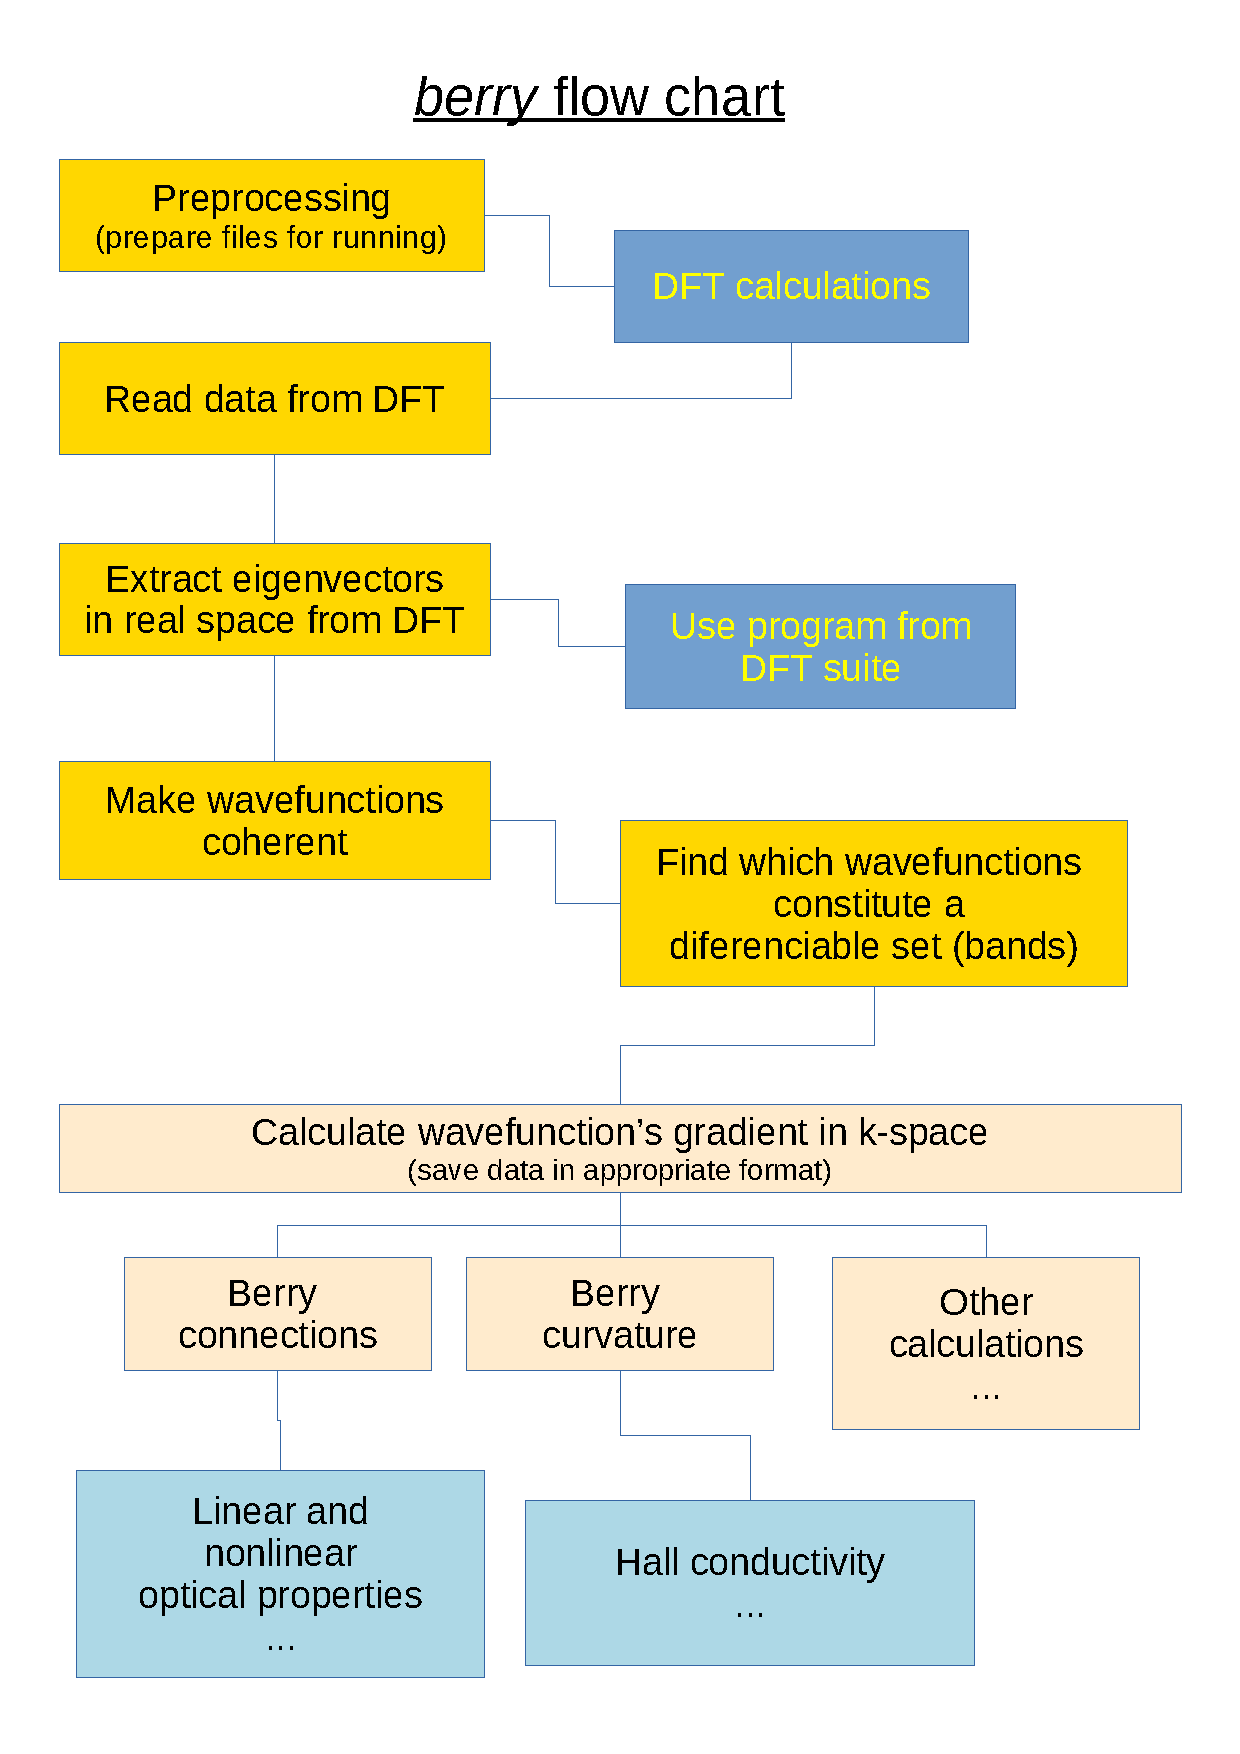
\includepdf[scale=0.8]{figures/berry_flow_chart.pdf}

The flowchart of the previous page explains how \textbf{berry} works.

First a preprocessing script is run which runs the DFT calculations, reads data from those
calculations, and saves it in files ready to be read by the folllowing scripts.

Then another script reads the wavefunctions from the DFT calculations and make them coherent.
This is done with the help of a script from the DFT suite.

The main part is the one that classifies each wavefunction into a band, assuring continuity.
Once this classification is done, the gradient in reciprocal space of the Bloch factors
of the wavefunctions can be calculated.

After that, Berry connections and curvatures, as well as other calculations can be performed.


\chapter{Theoretical background to \emph{berry}}

\section{Electronic structure calculations basics}

\subsection*{Crystal}
A crystal is a set of atoms, forming a pattern, that is replicated all over space in one, two or three dimensions.
It forms a crystal \emph{lattice}.

Here we will deal only with 2D materials, so the pattern, which is called \emph{unit cell},
is repeated in two dimensions, in a plane.

\begin{figure}
 \centering
 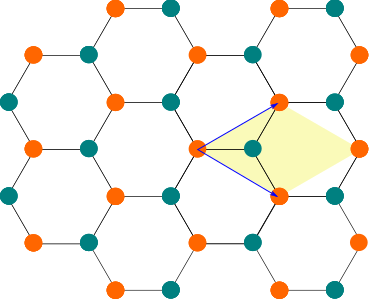
\includegraphics[scale=0.5,keepaspectratio=true]{figures/unitcell_honeycomb.png}
 \caption{Example of a unit cell in a two dimensional material, with hexagonal symmetry.
 The yellow shadow represents the unit cell and the two blue vectors represent the lattice vectors.}
 \label{fig:unitcell}
\end{figure}

The unit cell is defined by three vectors (two in 2D) $\pmb{a}_1$, $\pmb{a}_2$ and $\pmb{a}_3$,
in position space (the real space).
One can go from one unit cell to any other one by aplying the translation
\begin{equation}
 \pmb{R} = n_1\pmb{a}_1 + n_2\pmb{a}_2 + n_3\pmb{a}_3
\end{equation}
where $n_1$, $n_2$ and $n_3$ are integers, and $\pmb{R}$ is called the lattice vector.

A Fourier transform of this periodic pattern gives another periodic pattern in the so-called
\emph{reciprocal space} or momentum space.
This new periodicity is defined by the reciprocal vectors:
\begin{equation*}
 \pmb{b}_1 = 2\pi\dfrac{\pmb{a}_2\times\pmb{a}_3}{\pmb{a}_1\cdot (\pmb{a}_2\times\pmb{a}_3)};\hspace*{1cm}
 \pmb{b}_2 = 2\pi\dfrac{\pmb{a}_3\times\pmb{a}_1}{\pmb{a}_1\cdot (\pmb{a}_2\times\pmb{a}_3)};\hspace*{1cm}
 \pmb{b}_3 = 2\pi\dfrac{\pmb{a}_1\times\pmb{a}_2}{\pmb{a}_1\cdot (\pmb{a}_2\times\pmb{a}_3)}
\end{equation*}

\subsection*{Electrons in a crystal}

Electrons in a crystal can be described by the solutions to time independent Schr\"odinger equation:
\begin{equation}\label{eq:Schrodinger}
 H_{\pmb{k}}\psi_{\pmb{k},s}(\pmb{r}) = E_{\pmb{k},s}\psi_{\pmb{k},s}(\pmb{r})
\end{equation}
where $H_{\pmb{k}}$ is the hamiltonean of the system, which has the periodicity of the crystal lattice,
and is a function of the momentum $\pmb{k}$.
For each $\pmb{k}$ we have an equation \ref{eq:Schrodinger} that gives a (infinite) set of solutions,
which are labeled by the letter $s$.

The eigenvalues are the energies $E_{\pmb{k},s}$ and the respective eigenvectors are the wavefunctions
$\psi_{\pmb{k},s}(\pmb{r})$.

For a periodic material, the solutions to equation \ref{eq:Schrodinger} are given by Bloch's theorem:
\begin{equation}
 \psi_{\pmb{k}s}(\pmb{r}) = e^{i\pmb{k}\cdot\pmb{r}}u_{\pmb{k}s}(\pmb{r})
\end{equation}
with
\begin{equation}
 u_{\pmb{k}s}(\pmb{r}) = u_{\pmb{k}s}(\pmb{r} + \pmb{R})
\end{equation}
and $\pmb{k}$ is a point within the Brillouin Zone (BZ) and $s$ numbers the bands.
$\pmb{R}$ is the lattice vector.

$u_{\pmb{k}s}(\pmb{r})$ is called the Bloch factor and $e^{i\pmb{k}\cdot\pmb{r}}$
is called the Bloch phase factor.


\subsection*{Bands}

In the previous subsection the solutions of the Schr\"odinger equation were ordered by a \emph{band} index $s$.
In practice, the eigenvectors and eigenvalues are ordered in increasing energy, so that $E_{\pmb{k},0}$ is
the lowest energy solution of equation \ref{eq:Schrodinger}, $E_{\pmb{k},1}$ is the second lowest energy solution,
and so on.

Actually, there are a number of property calculations where it is necessary to use the set of eigenvectors
and eigenvalues that form a band as an entity in which mathematical operators must be applied
(the gradient in momentum space, for instance).
The Berry connection is an example.
The Berry connection is defined as:
\begin{equation}\label{eq:berry}
 \pmb{\xi}_{\pmb{k}ss'} = i\langle u_{\pmb{k}s}|\nabla_{\pmb{k}} u_{\pmb{k}s'} \rangle
                          = \dfrac{i}{v_C}\int_{uc} d^3\pmb{r}u_{\pmb{k}s}^*(\pmb{r})
                          \nabla_{\pmb{k}} u_{\pmb{k}s'}(\pmb{r})
\end{equation}
where $v_C$ is the volume of the unit cell and $uc$ stands for unit cell.

But the ordering (and grouping) of eigenstates by energy fails to give an usable entity for a gradient calculation,
because it frequently has discontinuities, i.e. is non-analytic.
\begin{figure}
 \centering
 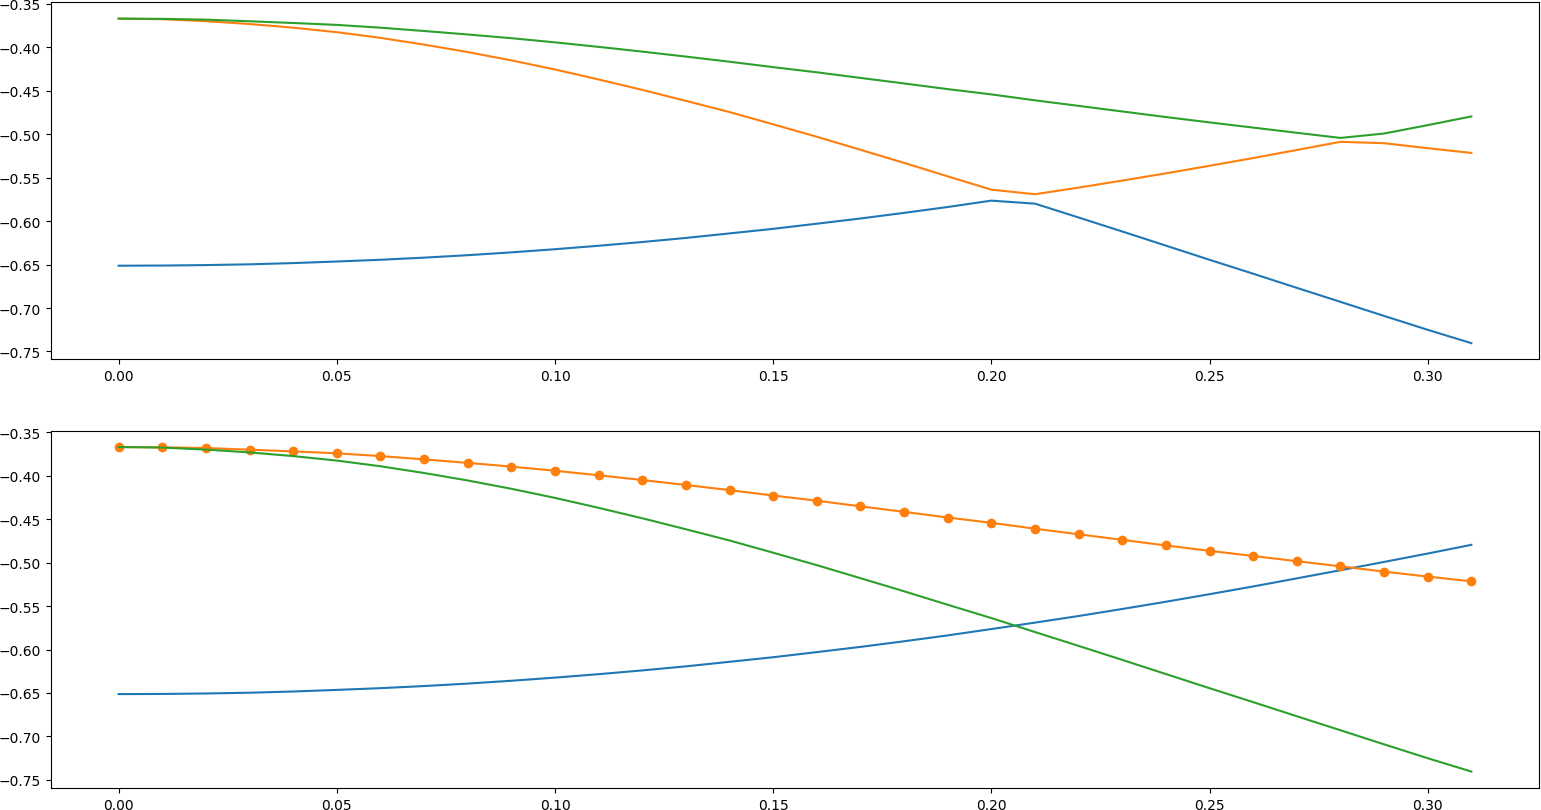
\includegraphics[scale=0.3,keepaspectratio=true]{figures/order_bands1D.png}
 % order_bands1D.png: 1541x810 px, 100dpi, 39.14x20.57 cm, bb=0 0 1110 583
 \caption{Example of electronic bands in one dimension.
 Different colors indicate different bands.
 Top: the bands according to the DFT output, that is, ordered by energy.
 Bottom: the bands according to continuity of the Bloch factors.
 The dots on the orange curve in the bottom figure indicate the positions of the k point sampling.}
 \label{fig:orderbands}
\end{figure}
Figure \ref{fig:orderbands} ilustrates the problem.
Where actual bands cross, the simple energy ordering cannot keep with the right band and jumps to another,
leading in fact to a discontinuity.

In order to be able to apply a gradient in momentum space we need to have the eigenstates ordered and grouped
in such a way that analycity is guaranteed.
That is the first goal of this suite of programs.



\subsection*{Band crossings}\label{ssec:bandcrossings}

It is clear that the problem of classifying the eigenstates by bands where analycity applies is
 problematic at degeneracies i.e. band crossings.

There, any linear combination of eigenstates is also an eigenstate.

Lets consider two bands $A$ and $B$, crossing at point $k$.
The eigenstates of $A$ are continuous at the left of $k$ and at the right, and the same is true for eigenstates of $B$.
But not necessarily at $k$.
Supppose that $\psi_A$ would be the wavefunction at $k$ that would have continuity in band $A$
and $\psi_B$ for band $B$. Of course, $\psi_A$ and $\psi_B$ have the same eigenvalue.

But the numerical process of solving the Schr\"odinger equation at point $k$ can give any result of the form
\begin{align}
 \psi_1 &= a\psi_A + b\psi_B \\
 \psi_2 &= a'\psi_A + b'\psi_B
\end{align}
as long as $\psi_1$ and $\psi_2$ are orthogonal (the coeficcients have to be such that they assure orthogonality).
Of course, these wavefunctions are not continuous with $A$ or $B$, in general.

There are two ways to workaround this problem and restore analycity.
One is to interpolate the wavefunction at $k$ using the closest eigenstates of band $A$ and then the ones of band $B$.
The other is to apply an unitary transformation.


\paragraph*{Unitary transformation}
The most frequent way of restoring analycity is to apply an unitary transformation
\begin{equation}
 \left[ \begin{matrix}
  \psi_A\\\psi_B
 \end{matrix}\right] = U
 \left[ \begin{matrix}
  \psi_1\\\psi_2
 \end{matrix}\right]
\end{equation}
where $U$ is choosen in such a way as to 'iron out' the nonanalytic behaviour at $k$.
In practice, this is done by minimizing the difference betwenn $\psi_A$ and both $\psi_A^-$ and $\psi_A^+$,
and the same for $\psi_B$ relative to $\psi_B^-$ and $\psi_B^+$.


\section{Graph Theory (GT)}

Graph Theory (GT) studies the properties and the applications of a mathematical structure called a Graph.
In a strict sense, a set of vertices (nodes) $V$ and a set of edges $E$ describes a Graph, $G(V, E)$.
A vertex (node), $v\in V$, is a terminal point, and an edge, is a link between two nodes.
This link must follow some relation, $R(v_1, v_2)$, between these nodes, for example, a co-authorship (edge) between two authors (nodes).

The edges are the set defined by
\begin{equation}
    E = \left\{(v_1, v_2) : v_1, v_2 \in V \wedge \exists\, R(v_1, v_2)\right\}
\end{equation}

The edges are oriented when the relationship between two nodes are diferent in each direction ($R(v_1, v_2) \neq R(v_2, v_1)$).
Thus, the graph is a directed graph, for example, the papers' citations (one paper cites another, but the opposite is not true).
However, if all pairs of nodes have the same edge in both directions ($ R(v_1, v_2) = R(v_2, v_1)$) or the orientation is irrelevant, its graph is undirected.

Furthermore, all relations need not have the same weight. For example, getting back to the co-authorship graph, some authors may collaborate more times with a few than others.
Thus, the edge between these two authors may include this weight $\omega(v_1, v_2)$ (it is a weighted graph).
Nonetheless, if the weights $\omega_e$ of all edges $e$ are the same ($\forall\, e\in E\; : \;\omega_e = \omega$) or the edges expresse a binary relation (may exist or not), the graph is unweighted.
In this work, we will use unweighted and undirected graphs.

Another essential concept is that of the subgraph.
A subgraph $g(V^\prime, E^\prime)$ is a graph formed by a subset of vertices $V^\prime \subset V$ and edges $E^\prime \subset E$ of a bigger graph $G(V, E)$.

A subgraph $g$, whose nodes do not have any edge between nodes of another subgraph $g^\prime, g \neq g^\prime$ is called a component.

Graph theory is very well studied, and there are many implemented algorithms to study graphs' properties.
We will use the \textit{networkx} python module for the implementation and analysis of graphs.



\section{Unsupervised Machine Learning (UML)}

AI solves problems that normally require a human to make decisions.
The cornerstone of Artificial Intelligence is designing agents that learn how to make informed decisions in possibly ever-changing environments without human supervision. Machine learning is a subset of AI where models learn patterns from datasets.
How an artificial agent learns these patterns classifies them into Supervised or Unsupervised machine learning (UML) models.

Unlike supervised machine learning, which uses data labeled by an expert and learned patterns from comparison, UML algorithms are used for clustering or association because they identify patterns from uncategorized data.
These algorithms recognize patterns in the datasets using some metrics to evaluate differences or similarities between data.

UML algorithms for clustering use a dataset of uncategorized points, and a  problem dependent metric.
The algorithm processes the points to form groups (clusters) represented by some pattern or structure determined by the metric.
The algorithm is called exclusive when a datapoint belongs exclusively to a single cluster.
The band-crossing problem lies in this class of algorithms due to its structure.
Thus, we will work with this type of clustering algorithm.






\chapter{Workflow}\label{ch:workflow}



\section{Preprocessing}\label{sec:preprocessing}
 After creating the files and directories mentioned in section \nameref{sec:running}, the next thing is
 to run the script \texttt{preprocess},
 \begin{verbatim}
  berry preprocess input_file [script options]
 \end{verbatim}
 which will do the following:
 \begin{enumerate}
  \item Reads file \texttt{inputfile} with the description of the run wanted.
  \item Runs the scf calculation using {\sc Quantum Espresso}, if it has not ran before.
  \item Generates an nscf input file according to the input file and runs an nscf calculation,
  using {\sc Quantum Espresso}, if it has not ran before.
  \item Reads data from the nscf calculation and saves to a file.
  \item Makes several simple calculations that will be used afterwards in other scripts,
  and save them to several files.
 \end{enumerate}

 An input file for the berry run has to be created in the working directory with several parameters.
The minimum parameters needed are:
\begin{itemize}
 \item origin of k-points (k0)
 \item number of k-points in each direction (nkx, nky, nkz)
 \item step of the k-points (step)
 \item number of bands to be calculated (nbnd)
\end{itemize}

An example of the minimum input file is shown in figure \ref{code:inputfile}.
A full list of the parameters that are accepted with the respective defaults (if any)
is shown in table \ref{tab:variables_preprocessing}.
There is a unique reference number that is attributed when running \texttt{preprocess},
that can be changed in the input file, but is not recomendable, because it is too easy to forget
to change that variable in the input file and attribute the same value for different runs.

\begin{figure}[h]
 \centering
\begin{verbatim}
  k0 0.00 0.00 0.00
  nkx 100
  nky 100
  nkz 1
  step 0.005
  nbnd 8
\end{verbatim}
\caption{Example of input file for \texttt{preprocess}.}
\label{code:inputfile}
\end{figure}



\begin{table}[h]
 \centering
 \caption{List of variables for the input file of \texttt{preprocess}.}

 \begin{tabularx}{\textwidth}{Xl}
 \textbf{Role of keyword}                     & \textbf{Variable (and defaults)}\\
\hline
 origin of k-points (3 real numbers)           & k0 \\
 number of k-points in each direction (integer)& nkx, nky, nkz \\
 step of the k-points (real number)            & step \\
 number of bands to be calculated (integer)    & nbnd \\
 \hline
 number of processors                         & npr = 1 \\
 dft directory                                & dftdirectory = 'dft/' \\
 scf file name                                & name\_scf = 'scf.in' \\
 directory where wavefunctions will be saved  & wfcdirectory = 'wfc/' \\
 point in real space where all phases match   & point = 1.178097 \\
 software for DFT                             & program = 'QE' \\
 Unique reference of run                      & refname = date and time \\
%  DFT prefix  & prefix = '' \\
%  DFT output directory & outdir = ''\\
 \hline
\end{tabularx}
 \label{tab:variables_preprocessing}
\end{table}





The script \texttt{preprocess} creates the files:
\begin{itemize}
 \item \emph{phase.npy}
 \item \emph{neighbors.npy}
 \item \emph{eigenvalues.npy}
 \item \emph{occupations.npy}
 \item \emph{positions.npy}
 \item \emph{kpoints.npy}
 \item \emph{nktoijl.npy}
 \item \emph{ijltonk.npy}
\end{itemize}
and \emph{datafile.npy} which is the main data file.

File \emph{neighbors.npy} lists the neighbors of each k-point
(which neighbors to consider may be an input parameter in the future).

File \emph{phase.npy} saves for each (k,r) the phase factor of the Bloch functions.

This finishes the preparatory phase.
The options for \texttt{preprocess} are shown in table \ref{tab:options_preprocess}.

\begin{table}[h]
 \centering
 \caption{Options for script \texttt{preprocess}}\label{tab:options_preprocess}
\begin{tabular}[]{lr}
\hline
  \texttt{-h}, \texttt{--help}  &\hspace*{2cm} Show a help message and exit \\
  \texttt{-o file\_path}        & Name of output log file\\
                                & Extension will be ignored \\
  \texttt{-flush}               & Flush the ouput to stdout \\
  \texttt{-v}                   & Increase output verbosity \\
  \hline
\end{tabular}
\end{table}


\section{Extraction of wavefunctions}

The next step is to extract the wavefunctions from the format used in the DFT package
(in this case it is {\sc Quantum Espresso}),
make them coherent and save them in a format adequate for the \textbf{berry} suite.

The script that does this job is \texttt{wfcgen}:
\begin{verbatim}
  berry wfcgen [script options]
\end{verbatim}

It uses the package wfck2r.x of the {\sc Quantum Espresso} suite to extract and save the wavefunctions
from the original format to a numpy file, in position space, one for each k-point and band.
It uses the same number of processes as used before in the DFT calculations.

After extracting the wavefunctions,
 a point in position space is choosen (see table \ref{tab:variables_preprocessing}),
away from points of high symmetry, and all wavefunctions
are multiplied by a phase such that at that point all have zero phase (are real).

The wavefunctions are then saved in the directory choosen to save them
(see table \ref{tab:variables_preprocessing}; default is \emph{working\_directory/}\emph{wfc/}),
and the files will be named in the form \emph{k0**b0XX.wfc} where \emph{**} is replaced by the number of the k point
and \emph{XX} is replaced by the number of the band.

Bands are as given by the DFT software i.e. ordered by energy,
and the lowest energy band is numbered zero and so on.

The options for \texttt{wfcgen} are shown in table \ref{tab:options_wfcgen}.
The default is to generate all formated wavefunctions, but for debugging it may be useful
to generate just for a singke k-point or a single wavefunction, for which we have the options
\texttt{-nk} and \texttt{-band} (has to be used in conjunction with \texttt{-nk}).

\begin{table}[h]
 \centering
 \caption{Options for script \texttt{wfcgen}}\label{tab:options_wfcgen}
\begin{tabular}[]{lr}
\hline
  \texttt{-nk}                  & Generates wavefunctions for a single k-point  \\
                                &  (default: All) \\
  \texttt{-band}                & Generates wavefunctions for a single k-point\\
                                &  and band (default: All) \\
  \texttt{-h}, \texttt{--help}  &\hspace*{2cm} Show a help message and exit \\
  \texttt{-o file\_path}        & Name of output log file\\
                                & Extension will be ignored \\
  \texttt{-flush}               & Flush the ouput to stdout \\
  \texttt{-v}                   & Increase output verbosity \\
  \hline
\end{tabular}
\end{table}


\section{Dot product}

\texttt{dot} reads the wavefunctions saved in directory \emph{wfc},
removes the phase factor of the Bloch functions, and calculates the dot product
of the Bloch factors of the neighboring k points.

\begin{verbatim}
  berry dot [script options]
\end{verbatim}

The neighboring k points are the four nearest neighbors, as determined in the preprocessing
and saved in file \emph{neighbors.npy}.

In the end we get two files \emph{dpc.npy} and \emph{dp.npy}:
\begin{itemize}
 \item \emph{dpc.npy} contains for each pair of k-points and bands the dot product of the Bloch factors
 \item \emph{dp.npy} contains the modulus of \emph{dpc.npy}
\end{itemize}
The options for \texttt{dot} are shown in table \ref{tab:options_dot}

\begin{table}[h]
 \centering
 \caption{Options for script \texttt{dot}}\label{tab:options_dot}
\begin{tabular}[]{lr}
\hline
  \texttt{-h}, \texttt{--help}  &\hspace*{2cm} Show a help message and exit \\
  \texttt{-np}                  & Number of processes to use (default: 1) \\
  \texttt{-o file\_path}        & Name of output log file.\\
                                & Extension will be ignored. \\
  \texttt{-flush}               & Flush the ouput to stdout \\
  \texttt{-v}                   & Increase output verbosity \\
  \hline
\end{tabular}
\end{table}



\section{Find the bands}
To find which eigenvalues/eigenfunctions have continuity, one runs script \texttt{cluster}.

\begin{verbatim}
  berry cluster [script options]
\end{verbatim}

This script uses graph theory and unsupervised machine learning to establish electronic bands
that are analytic in k-space.

It uses data from files \emph{dp.npy} and \emph{eigenvalues.npy} to establish continuity
between wavefunctions of neighboring k-points.

 It retrieves two files:
 \begin{description}
   \item[\emph{bandsfinal.npy}] stores an array bandsfinal[k,b] = number of band that is continuous to band b.
   \item[\emph{signalfinal.npy}] signalfinal[k,b] is a measure of the quality of the attribution to a band.
 \end{description}

 A detailed explanation of the algorithm is given in the appendix \nameref{cha:cluster}.

 The options for \texttt{cluster} are shown in table \ref{tab:options_cluster}.

\begin{table}[h]
  \centering
  \caption{ Options for script \texttt{cluster}}\label{tab:options_cluster}
  \begin{tabular}[]{lr}
  \hline
  \texttt{-h}, \texttt{--help}  & Show a help message and exit \\
  \texttt{-mb}                  & Minimum band to consider (default: 0) \\
  \texttt{-np}                  & Number of processes to use (default: 1) \\
  \texttt{-t [0.0-1.0]}         & Tolerance used for graph construction (default: 0.95) \\
  \texttt{-o file\_path}        & Name of output log file\\
                                & Extension will be ignored \\
  \texttt{-flush}               & Flush the ouput to stdout \\
  \texttt{-v}                   & Increase output verbosity \\
  \hline
 \end{tabular}
 \end{table}



\section{Basis rotation}
 It is frequent that a basis rotation has to be applied to some wavefunctions in such a way
 as to maximize continuity, where there is a degeneracy.

 For this, \texttt{basis} can be run.

 \begin{verbatim}
  berry basis [script options]
 \end{verbatim}

 It works like this:
 Consider a point in k-space and two wavefunctions $|\Psi_1\rangle$ and $|\Psi_2\rangle$
 that have been signaled as not continuous to the neighboring wavefunctions $|\Psi_A\rangle$ and $|\Psi_B\rangle$
 that belong to band $A$ and band $B$, respectively.

 We will apply an unitary transformation
 \begin{align*}
  |\Psi_A'\rangle &= a_1|\Psi_1\rangle + a2|\Psi_2\rangle \\
  |\Psi_B'\rangle &= b_1|\Psi_1\rangle + b2|\Psi_2\rangle
 \end{align*}
 where we have the restrictions due to orthonormalization:
 \begin{align*}
  a_1a_1^* + a_2a_2^* &= 1\\
  b_1b_1^* + b_2b_2^* &= 1\\
  a_1^*b_1 + a_2^*b_2 &= 0
 \end{align*}

 Then we want this transformation to be such that maximizes continuity to bands $A$ and $B$, so we want
 the dot products $\langle \Psi_A|\Psi_A'\rangle $ and $\langle \Psi_B|\Psi_B'\rangle $ to be close to $1$,
 which is the maximum they can be.

 We look for the set $a_1, a_2, b_1, b_2$ that give
 \begin{align*}
  \max \langle \Psi_A|\Psi_A'\rangle &= \max \left( \langle \Psi_A|\Psi_1\rangle a_1 + \langle \Psi_A|\Psi_2\rangle a_2\right) \\
  \max \langle \Psi_B|\Psi_B'\rangle &= \max \left( \langle \Psi_B|\Psi_1\rangle b_1 + \langle \Psi_B|\Psi_2\rangle b_2\right)
 \end{align*}

 It will create new wavefunctions with extension \emph{.wfc1}, that will be used in subsequent calculations.
The options for \texttt{basis} are shown in table \ref{tab:options_basis}

\begin{table}[h]
 \centering
 \caption{Options for script \texttt{basis}}\label{tab:options_basis}
 \begin{tabular}[]{lr}
 \hline
  \texttt{-h}, \texttt{--help}  &\hspace*{2cm} Show a help message and exit \\
  \texttt{-np}                  & Number of processes to use (default: 1) \\
  \texttt{-o file\_path}        & Name of output log file\\
                                & Extension will be ignored \\
  \texttt{-flush}               & Flush the ouput to stdout \\
  \texttt{-v}                   & Increase output verbosity \\
  \hline
 \end{tabular}
\end{table}


\section{Convert wavefunctions to k space}

With the bands well defined, it is now necessary to proceed to calculate the wavefunctions in k-space and their gradients.

For that, run \texttt{r2k}:
\begin{verbatim}
  berry r2k highest_band [script options]
 \end{verbatim}

It will calculate from band 0 to the value of the band given (\texttt{highest\_band}),
unless a minimum band is given.
The highest band has to be given because in principle not all bands that were initialy calculated will
be complete, and it doesn't make sense to use them in further calculations.

The wave functions originaly are saved for each k-point in a file, and the file contains the value of the wavefunction in each
point of the real space.
This program converts this format to one where for each point in real space there is a file with all the values of wavefunctions
of the same band as a function of k-points, which is suitable to diferentiate.
\begin{equation*}
 \Psi_{\pmb{k}}(\pmb{r}) \rightarrow \Psi_{\pmb{r}}(\pmb{k})
\end{equation*}

Will save the wavefunctions of each band in a compressed file \emph{wfcpos\#.npy} where \# = number of band
and the gradients of each band in a compressed file \emph{wfcgra\#.npy} where \# = number of band.
The options for \texttt{r2k} are shown in table \ref{tab:options_r2k}.

\begin{table}[h]
 \centering
 \caption{Options for script \texttt{r2k}}\label{tab:options_r2k}
\begin{tabular}[]{lr}
\hline
  \texttt{-h}, \texttt{--help}  &\hspace*{2cm} Show a help message and exit \\
  \texttt{-np}                  & Number of processes to use (default: 1) \\
  \texttt{-mb}                  & Minimum band to consider (default: 0) \\
  \texttt{-o file\_path}        & Name of output log file\\
                                & Extension will be ignored\\
  \texttt{-flush}               & Flush the ouput to stdout \\
  \texttt{-v}                   & Increase output verbosity \\
  \hline
\end{tabular}
\end{table}



\section{Calculation of the Berry connections and curvatures}

The Berry connections (equation \ref{eq:berry}) and curvature are calculated using the script \texttt{geometry}.
\begin{verbatim}
  berry geometry highest_band [script options]
 \end{verbatim}


The highest band is the number of the last band to be used in the calculations.
In principle, it will be the same as the one used in \texttt{r2k}.
The options for \texttt{geometry} are shown in table \ref{tab:options_geometry}.

\begin{table}[h]
 \centering
 \caption{Options for script \texttt{geometry}}\label{tab:options_geometry}
\begin{tabular}[]{lr}
  \hline
  \texttt{-h}, \texttt{--help}  &\hspace*{2cm} Show a help message and exit \\
  \texttt{-np}                  & Number of processes to use (default: 1) \\
  \texttt{-mb}                  & Minimum band to consider (default: 0) \\
  \texttt{-prop} [both,connection,curvature] &  Specify which property to calculate. (default: both)\\
  \texttt{-o file\_path}        & Name of output log file\\
                                & Extension will be ignored\\
  \texttt{-flush}               & Flush the ouput to stdout \\
  \texttt{-v}                   & Increase output verbosity \\
  \hline
\end{tabular}
\end{table}



\section{Optical conductivity and second harmonic generation}

To calculate the linear condutivity, the script \texttt{condutivity} should be used
and for the second harmonic condutivity, the script \texttt{shg}.
\begin{verbatim}
  berry conductivity highest_band [script options]
 \end{verbatim}
 and
 \begin{verbatim}
  berry shg highest_band [script options]
 \end{verbatim}

The highest band is the number of the last band to be used in the calculations,
and has to be higher than the valence band.
There are several options for the calculation that can be changed and are listed in
table \ref{tab:options_conductivity}.


\begin{table}[h]
 \centering
 \caption{Options for scripts \texttt{conductivity} and \texttt{shg}.}\label{tab:options_conductivity}
\begin{tabular}[]{lr}
\hline
  \texttt{-h}, \texttt{--help}  & Show a help message and exit \\
  \texttt{-np}                  & Number of processes to use (default: 1) \\
  \texttt{-eM}                  & Maximum energy in Ry units (default: 2.5) \\
  \texttt{-eS}                  & Energy step in Ry units (default: 0.001) \\
  \texttt{-brd}                 & Energy broading in Ry units (default: 0.01) \\
  \texttt{-o file\_path}        & Name of output log file\\
                                & Extension will be ignored\\
  \texttt{-flush}               & Flush the ouput to stdout \\
  \texttt{-v}                   & Increase output verbosity \\
  \hline
\end{tabular}
\end{table}

These scrips calculate the conductivity between 0 and the maximum energy (in Ry),
with a step (energy step) and a broadning.

The details of these calculations can be found in
\begin{verbatim}
 https://arxiv.org/abs/2006.02744
\end{verbatim}




\begin{appendices}

\chapter{Installing for noncolinear calculations}
\label{ch:noncolinear}
The installation can be replicated by following:
First, create a copy of \verb|wfck2r.f90| located in PP/src of the Quantum ESPRESSO's source code and name it \verb|wfck2rFR.f90| in the same directory.
In the wfck2rFR.f90 file, on line 252, between \verb|enddo| and \verb|endif|, add in new lines:
\begin{verbatim}
if (noncolin) then                      !added!
  do i3 = 1, dffts%nr3x, nevery(3)    !added!
  do i2 = 1, dffts%nr2x, nevery(2)    !added!
  do i1 = 1, dffts%nr1x, nevery(1)    !added!
    !val = local_average()          !added!
    val=dist_evc_r(i1+(i2-1)*dffts%nr1x+(i3-1)*dffts%nr1x*dffts%nr2x,2)    !added!
    write(iuwfcr+1,'("(",E20.12,",",E20.12,")")') val    !added!
  enddo    !added!
  enddo    !added!
  enddo    !added!
endif        !added!
\end{verbatim}


Then on the same directory PP/src it is needed to edit the \verb|Makefile|.
On line  76, between \verb|wfck2r.x| and \verb|fermi_velocity.x| add in the same line \verb|wfck2rFR.x|.
Next, on the same \verb|Makefile|, add on line 175:

\begin{verbatim}
wfck2rFR.x : wfck2rFR.o libpp.a $(MODULES)
        $(LD) $(LDFLAGS) -o $@ \
                wfck2rFR.o libpp.a $(MODULES)  $(QELIBS)
        - ( cd ../../bin ; ln -fs ../PP/src/$@ . )
\end{verbatim}

After this, to compile, just execute the command on the directory PP/src:

\begin{verbatim}
    make wfck2rFR.x
\end{verbatim}


\chapter{Glossary}

This glossary indicates the meaning of the variables used in the suite \textbf{berry}.
\vspace{0.5cm}

\begin{tabularx}{\textwidth}{Xl}
 npr            & Number of processors for the run \\

 nkx            & Number of k-points in the x direction \\
 nky            & Number of k-points in the y direction \\
 nkz            & Number of k-points in the z direction \\
 nks            & Total number of k-points \\

 nr1            & Number of points of wfc in real space x direction \\
 nr2            & Number of points of wfc in real space y direction \\
 nr3            & Number of points of wfc in real space z direction \\
 nr             & Total number of points of wfc in real space \\

 k0             & Initial k-point (coordinates) (2pi/bohr) \\
 step           & Step between k-points (2pi/bohr) \\
\end{tabularx}
\vspace{0.5cm}

\begin{tabularx}{\textwidth}{Xl}
 dftdirectory   & Directory of DFT files \\
 name\_scf       & Name of scf file (without suffix) \\
 name\_nscf      & Name of nscf file (without suffix) \\
 wfcdirectory   & Directory for the wfc files \\
 prefix         & Prefix of the DFT QE calculations \\
 outdir         & Directory for DFT saved files \\
 dftdatafile    & Path to DFT file with data of the run \\
 berrypath      & Path of BERRY files \\
\end{tabularx}
\vspace{0.5cm}

\begin{tabularx}{\textwidth}{Xl}
 a1             & First lattice vector in real space (bohr) \\
 a2             & Second lattice vector in real space (bohr) \\
 a3             & Third lattice vector in real space (bohr) \\

 b1             & First lattice vector in reciprocal space ($2\pi$/bohr) \\
 b2             & Second lattice vector in reciprocal space ($2\pi$/bohr) \\
 b3             & Third lattice vector in reciprocal space ($2\pi$/bohr) \\
\end{tabularx}
\vspace{0.5cm}

\hspace*{-2cm}\begin{tabularx}{\textwidth}{ll}
 nbnd           & Number of bands \\

 eigenvalues    & Array with all eigenvalues of the calculation (Ry) \\
 occupations    & Array with all occupations of the calculation \\

 phase[i,nk]    & Array with exp(1j*(kpoints[nk,0]*r[i,0] + kpoints[nk,1]*r[i,1] + kpoints[nk,2]*r[i,2])) \\
 kpoints[nk,2]  & Array with coordinates of all k-points ($2\pi$/bohr) \\
 r[i,2]         & Array with coordinates of all points of space (bohr) \\

 neig[nk,3]     & Array with number of the four k-points around nk \\
\end{tabularx}


\chapter{List of files in the suite}
 All programs of this package are in python 3.

The package contains the python scripts in the main berry directory:
\begin{itemize}
 \item preprocessing.py
 \item generatewfc.py
 \item dotproduct.py
 \item clustering\_bands.py
 \item basisrotation.py
 \item r2k.py
 \item berry\_geometry.py
 \item condutivity.py
 \item shg.py
\end{itemize}\medskip

and the auxiliary files:
\begin{itemize}
  \item cli.py
  \item \_\_init\_\_.py
  \item \_version.py
\end{itemize}\medskip


Visualization scripts are in directory 'vis':
\begin{itemize}
 \item \_debug.py
 \item \_geometry.py
 \item \_wave.py
\end{itemize}\medskip

Also the subroutines (depend on the other scripts) are in directory '\_subroutines':
\begin{itemize}
 \item headerfooter.py
 \item contatempo.py
 \item parserQE.py
 \item loaddata.py
 \item loadmeta.py
 \item comutator.py
 \item write\_k\_points.py
 \item clustering\_libs.py
 \item clustering\_signaling.py
\end{itemize}

Some utilities are in directory 'utils':
\begin{itemize}
  \item emailSender.py
  \item jit.py
  \item \_logger.py
\end{itemize}

It is likely that some of these scripts will be merged with others
while new ones will appear due to new functionalities.






\chapter{Algorithm of \texttt{cluster} script}
\label{cha:cluster}


    \section{Algorithm}
    This solution employs different techniques to solve the bands crossing problem as graph theory and unsupervised machine learning methods.
    The bands clustering algorithm uses the information of k-points' wavefunctions, the dot products of their Bloch factors, and their corresponding band energy.
    Thus, the solver algorithm iterates between two main pieces: the component identification based on graph theory and the samples assignment using unsupervised machine learning methods.

The solver's objective is to get closer to the best solution in each iteration by maximizing the number of solved bands.

The bands clustering algorithm uses the wave functions, their dot products, and their corresponding band energy for these calculations.

The output are five files that will be used by other programs, and will be described below.

In the following sections we will discuss in more detail the purpose of each band clustering algorithm's part and how it works.



\subsection{Problem configuration and notation definition}

We first need to organize the information problem in a convenient data structure.
The essential elements we have are the energies $E_{k,n}$ for each k-point $\vec{k}\equiv \left(k_x, k_y\right)$ and band $n$, the k-points' neighbor identification, and the dot product between the neighboring Bloch factors.
The \textit{loaddata} module gives the algorithm most of this information; however, this module does not contain the dot product data; it is in the \textit{dp.npy} file.

First, we create a mixed entity using a k-point and its band energy as if it were a vector on a "bands-energy" space.
In the following, a variable $\vec{p}$ identifies a point in this space.
Thus, this variable $\vec{p}$ contains the k-point coordinates and an eigenenergy of the k-point (which is a band designation).

\begin{equation}
    \vec{p} \equiv \left(k_x, k_y, E_{k,n}\right)
\end{equation}

The set of all k-points identifiers ($k$ indices) is $K$, where $K \equiv \left[k = 0,\dots,  N-1\right]$, and $\vec{K}\equiv \left\{\vec{k}_0, \vec{k}_1, \dots, \vec{k}_{N-1}\right\}$ is the set of all k-points vectors.
$N$ is the total number of k-points.
It is possible to define an index $p$ which uniquely determines a wavefunction' Bloch factors:
\begin{equation}
    p = n\, N + k
\end{equation}
We call $P$ to the set of all $p$'s.
$n$ is the original band as attributed by the DFT software; we define the set of $n$'s: $B\equiv\left[0, n_B-1\right]$.
$n_B$ is the total number of bands.


Then
\begin{equation}
    P \equiv \left[0, n_B N -1\right]
\end{equation}

It leads to
\begin{equation}
    E_{k,n} = E_p,\hspace{1cm} k\in K, \; n\in B,\; p\in P
\end{equation}

Let us consider the points $p$ and $q$ $\in P$, with $q$ is neighbor of $p$
(by neighbor we mean that the k-points that are implicit in the varaibles are adjacent in $x$ or $y$ directions in reciprocal space);
the dot product between their Bloch factors is given by $0\leq \left|\braket{p}{q}\right|< 1$.
If the Bloch factors $p$ and $q$ belong to the same band, and the band is analytic, since they are close together, their dot product should be close to one.
On the other hand, this dot product should be close to zero if $p$ and $q$ belong to different bands, since different bands are orthogonal.

Thus, this data seems to give all the information necessary to solve the band-crossing problem.
However, from a computational point of view, more is needed;
during the implementation of this solution, several problems were found, and just a few of them were solved successfully.

Regardless, the dot product information is not wholly needless for values close to one $\left|\braket{p}{q}\right|\approx 1$;
it is possible to form groups of well-constructed groups of points.
The existence of points and a way of measuring relations between them reminds the graph concept.
This is the motivation for one of the algorithm's parts:
use graph theory methods to identify these groups and, after that, use unsupervised machine learning techniques to classify them.

Consequently, this information makes it possible to construct the first data structure.
It is a graph $G(V, E)$ ($V$ is a set of vertices or nodes, and $E$ is a set of edges (connections)) where each point $p$ is a node, so that $V=P$, and if the connection (dot-product) is more significant than an adequate tolerance $\mathrm{TOL}$, there is an edge between these nodes.
For simplicity, this graph is undirected and does not have weights on its edges.

\begin{equation}
    E = \left\{(p,q)\;|\;p,q\in P \;\;\wedge\;\; \left|\braket{p}{q}\right| > \mathrm{TOL}\right\}
\end{equation}

Therefore, the initial state of the problem is prepared in a convenient data structures.
The next step is the solver algorithm that will use that data and the graph previously constructed as the initial solution point.
The solver algorithm will iterate over this information.

\subsection{Solver Algorithm}

The solver algorithm (SA) is an optimization process based on iteration for solving the band-crossing problem.
As discussed before, this algorithm iterates between two parts.
One piece is based on graph theory (GT), and the other is based on unsupervised machine-learning (UML) techniques.
The initial conditions for this algorithm were described in the previous section.
This SA follows the flux chart in figure \ref{fig:flux_chart}.


\begin{figure}
    \centering
    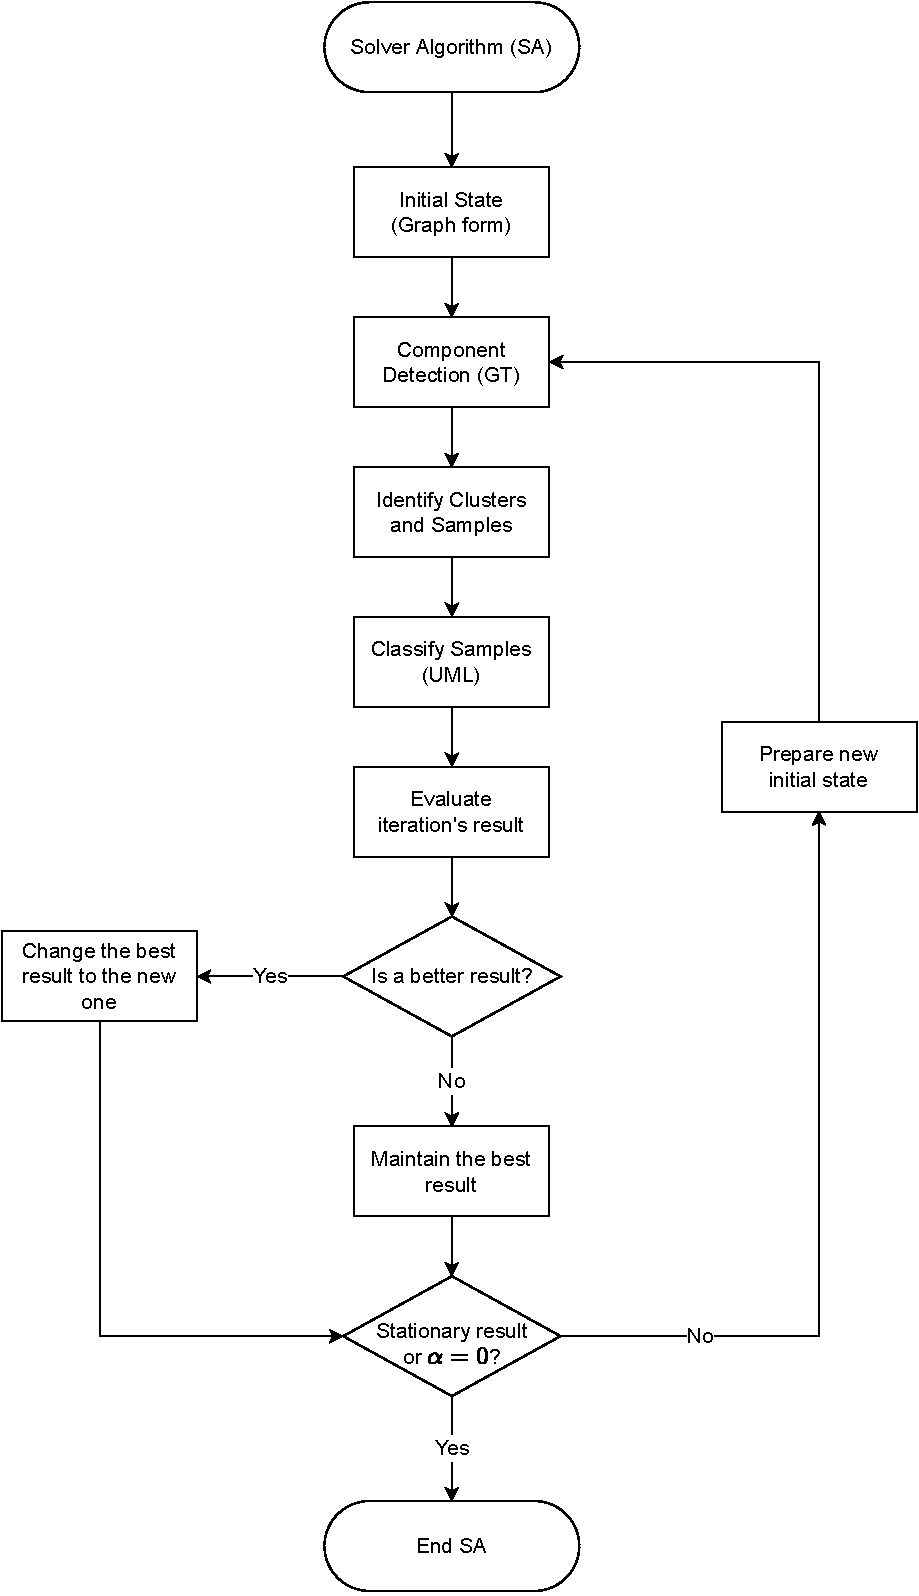
\includegraphics[width=0.8\textwidth]{figures/Fluxchart.pdf}
    \caption{Flowchart with a simplified description of the solver algorithm.}
    \label{fig:flux_chart}
\end{figure}


The SA can be simply described as various iterations starting in an initial state, and as a result some points are not attributed to their initial band and others are noted as having a strong connection between them.
We call components to the sets of points with connections and if there are no connections, the single point is also considered a component.
In the first iteration, these components were computed by constructing the graph using the dot-product information only.

The initial state of an iteration is the best result of the previous iterations, since SA  is an optimization algorithm.

One SA iteration involves identifying the components, given the initial state in the form of a graph.
Then, clustering these components gives larger components, that will form a new state that will be used as a initial state of the next iteration.
The optimization process ends when the result does not change between iterations, reaching a stationary solution or the relaxation parameter reaches the minimum value.
This relaxation value is a parameter for the second part of the algorithm, and will be discussed in more detail later.


\subsection{Identification of problems and component detection}

The concept of a component in GT is necessary to understand this part of the SA.
A component is a sub-graph (i.e., a smaller graph $g$ belonging to a bigger one $G$ where $g\subset G$), with edges (connections) between its nodes, but no connections with the nodes of other components, as shown in the example in figure \ref{fig:components}.


\begin{figure}
    \centering
    \begin{subfigure}[b]{0.45\textwidth}
        \centering
        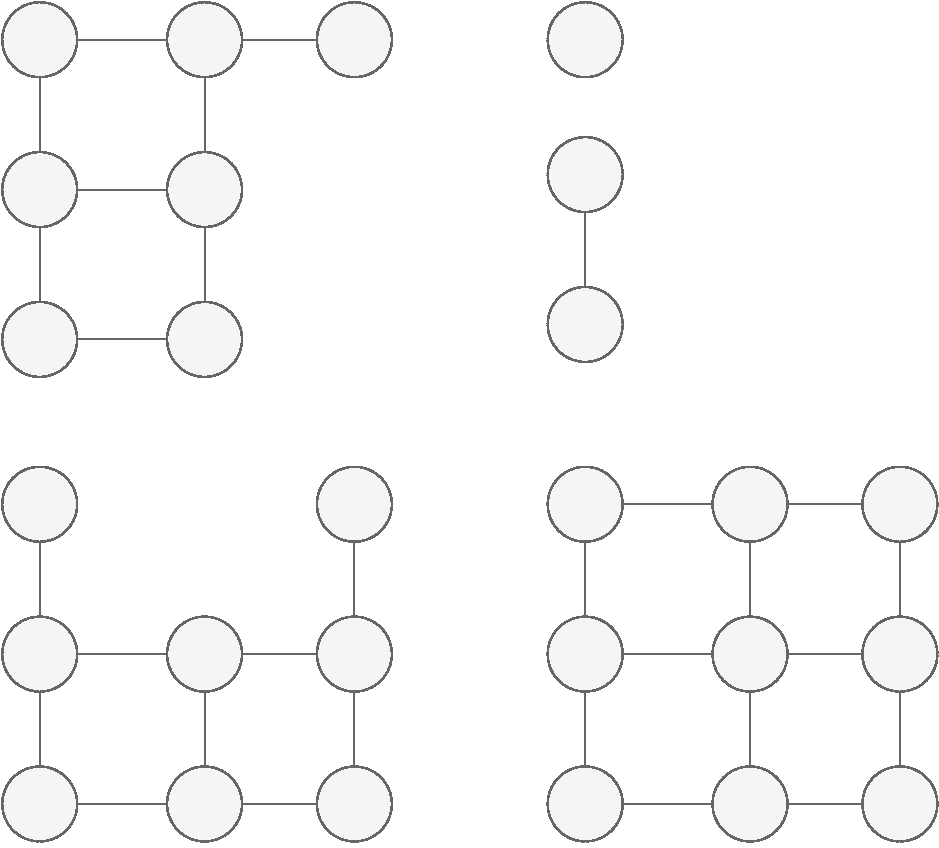
\includegraphics[width=\textwidth]{figures/Graph.pdf}
        \caption{}
        \label{fig:Ca}
    \end{subfigure}
    \hfill
    \begin{subfigure}[b]{0.45\textwidth}
        \centering
        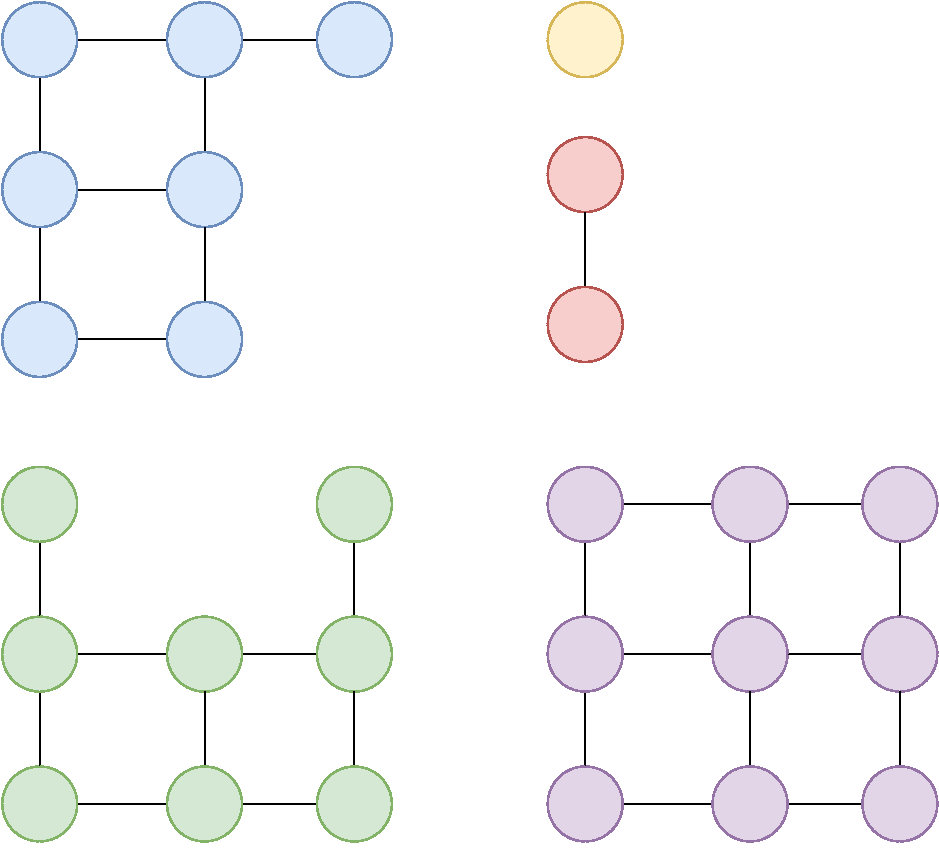
\includegraphics[width=\textwidth]{figures/Components.pdf}
        \caption{}
        \label{fig:Cb}
    \end{subfigure}
    \caption{Figure \ref{fig:Ca} represents a general graph $G(V, E)$ where the vertices $V$ are the gray circles, and the edges $E$ are the line that connects them. Figure \ref{fig:Cb} shows the $G$'s components. Each component is identified with a different color.}
    \label{fig:components}
\end{figure}

These components are straightforward to identify using existing GT techniques, but as expected, they are not the final result are just portions of a band.
For this reason, it is essential to classify these components to form completed bands.
Hence, the SA uses UML techniques to perform the assignment.

This algorithm gives very good results for some materials; however, there are problems.
Namely, a few points create "loops" between prohibited points.
It is a prohibited path because, there should be no connection between two points in the same k-point (that is two wavefunctions with the same k-point must not belong to the same band).
This results in the algorithm assuming two components that should be separated as a single component.


Two types of points create these "loops."
One of them is straightforward to identify; they are degenerate points up to a numerical error
(i.e., for $p$ and $q \in P$ and the same $k$-point, their energy is numerically the same, $E_p=E_q$).
Thus, it is only necessary to identify them and see if they create these forbidden paths.
When found, the connection is broken.

The second type of points are not strictly degenerate but have the same behavior, complicating their detection.
These more peculiar points are in high energy bands and, besides other inconveniences, limit the algorithm to obtain better results.
Nonetheless, for both types of problems, we need a more substantial justification for this behavior.




\subsection{Unsupervised Machine Learning Techniques to Band Clustering}

Since the SA uses UML techniques to classify the components, it is necessary to establish a clear notation.
We call clusters the components with many points that can not join to another large component, because they are geometricaly incompatibles.
These clusters are electronic bands of eingenenergies with part of their points attributed.
We call samples to the rest of components, that can be assigned to clusters.
When a cluster has the number of nodes (points $p$) equal to the total number of $k$-points, $N$, this cluster is solved (the band is solved). Otherwise, it is an incomplete cluster, and the sample assignment tries to complete it.

Supervised machine learning methods require large quantities of labeled examples, which we do not have. Thus, this problem lies in the unsupervised machine learning (UML) problems category. Consequently, this SA's part aims to identify the samples that complete the clusters using these UML methods.

The UML method needs a way to compare samples to clusters and evaluates the attribution. Therefore, let us define the similarity between two objects, $\mathrm{X}$ and $\mathrm{Y}$, $\mathcal{S}(\mathrm{X}, \mathrm{Y})$. The $\mathcal{S}(\mathrm{X}, \mathrm{Y})$ value measures how similar these objects are based on one chosen metric. When the similarity is higher, the objects are more similar. We will use a normalized similarity.
So, the $\mathcal{S}$ value must satisfy the following properties:

\begin{enumerate}
    \item It is positive, $\mathcal{S}(\mathrm{X}, \mathrm{Y}) > 0$
    \item It is symetric, $\mathcal{S}(\mathrm{X}, \mathrm{Y}) = \mathcal{S}(\mathrm{Y}, \mathrm{X})$
    \item It is maximum when $\mathrm{X}=\mathrm{Y}$, $\mathcal{S}(\mathrm{X}, \mathrm{X})=1$
\end{enumerate}

On the other hand, we use a similarity metric between samples and clusters that only needs their representative points. A cluster has many well-connected points, but only a few are required for comparison with a candidate sample to join the cluster. Only the cluster and sample boundary points may establish relations between them. Then, these are the representative points.

Identifying the representative points is an undersampling technique.
We use the convolution of the Prewitt operator, $(G_x, G_y)$, with the cluster's k-space projection $A$ to determine their edges.
The matrix $A$ has the shape of k-space; each matrix's entry, $A_{k_x,k_y}$, is one if the cluster includes a point $\vec{p}(p)$ with that $k$-point and zero otherwise.

 This operator is a simple discrete gradient that identifies high-frequency variations. These variations define the cluster's edges.


\begin{equation}
    A_{k_x,k_y} = \left\{
    \begin{array}{cc}
        1, & \vec{k} \in \vec{K}_\text{Cluster}\subset \vec{K} \\
        0, & \text{otherwise}
    \end{array}
    \right.
\end{equation}

The Prewitt operator $G_x$ and $G_y$ is defined as:

\begin{multicols}{2}
    \begin{equation}
        G_x = \left[
            \begin{array}{ccc}
                -1 & 0 & 1 \\
                -1 & 0 & 1 \\
                -1 & 0 & 1
            \end{array}
            \right]
    \end{equation}
    \begin{equation}
        G_y = G_x^T=\left[
            \begin{array}{ccc}
                -1 & -1 & -1 \\
                0  & 0  & 0  \\
                1  & 1  & 1
            \end{array}
            \right]
    \end{equation}
\end{multicols}

Then, the gradient on the $\alpha=\{x,y\}$ direction of $A$ is

\begin{equation}
    A_\alpha = G_\alpha \ast A,\hspace{1.5cm}\alpha=\{x,y\}
\end{equation}
where $\ast$ is the convolution operator and the representative cluster edges are given by.

\begin{equation}
    \text{edges} = \sqrt{A_x^2+A_y^2} > 0
\end{equation}

Now, we can explicitly choose a metric to define the similarity that we will use.
A similarity score between neighboring representative points is a weighted mean between the modulus of the dot product $\left|\braket{p}{q}\right|$, and a function $f_p(E_q)$ of the energies $E_q$ of the neighbor point $q$.

The similarity of a cluster with a sample is defined as the mean of the individual similarity score between neighboring representative points.

Thus, the similarity score, $s_p^q$, between the cluster's $p\in P$ point and its sample's $q \in P$ neighbor is:

\begin{equation}
    s_p^q = \alpha\left|\braket{p}{q}\right| + \left(1-\alpha\right)f_p(E_q)
\end{equation}

The value of $\alpha$ is a relaxation parameter in the optimization process.
Its initial value is $1/2$, and it diminishes on each iteration.
The $\alpha$'s minimum value is $0$ due to normalization.
The function $f_p(E_q)$ computes the normalized difference between the best-expected energy $E_{\text{best}}$ with the actual $q$'s energy, $E_q$.

\begin{equation}
    f_p(E_q) = \frac{\text{min}\{\Delta E_\text{best}^{i}\}_i}{\Delta E_\text{best}^q},\hspace{1.5cm} \Delta E_a^b = |E_a-E_b|
\end{equation}
\begin{equation}
    i \in \left\{n N + k: \forall_n\hspace{0.2cm}n\in B\right\}
\end{equation}

We consider a smooth variation of bands in bands-energy space. Thus, the energy profile in each band's $\vec{p}$ point can be approximated by a second-order polinomial. This approximation allows us to calculate the best energy value $E_\text{best}$ by extrapolation from the neighboring points that belong to the cluster.
If there are not enough points to fit the curve, the $p$'s energy is used,  $E_\text{best}=E_p$.

Comparing all possible energy values $E_i$ for the corresponding $q$'s $k$-point $k$, the value that minimizes the difference with the best energy is obtained.




Then, the similarity $\mathcal{S}(\mathrm{C},\mathrm{S})$ between the cluster $\mathrm{C}$ and sample $\mathrm{S}$  is

\begin{equation}
    \mathcal{S}(\mathrm{C},\mathrm{S}) = \frac{1}{4\tilde{N}}\sum_{p\in \mathrm{C}}\sum_{q\in\mathrm{S}} s_p^q,\hspace{1.5cm}\mathrm{C},\mathrm{S}\subset P
\end{equation}

Where $\tilde{N}$ is the total number of points in the sample's edge. The factor of 4 appears because each $q$ point generally contains four neighbors.

Assigning samples to clusters uses similarity values, trying to maximize it between them.
Hence, all the samples are compared to all clusters to obtain their similarities. The classification is made iteratively. For each iteration, one sample is assigned to the best cluster. After that, the similarity scores are recalculated between the samples and the modified cluster.

This UML algorithm is the SA's bottleneck in executing time. This complication comes from the fact that this part is mostly computed linearly (i.e., the result on each iteration depends on the previous result). Therefore parallelizing it is challenging.

Ultimately, all the samples are assigned to one cluster leading to a band solution.
However, as mentioned before, many problematic points exist.
In particular, high energy bands usually have many oscilations, and in this case the assumption of smooth variation is inaccurate, and the metric criteria has to be improved.





\subsection{Evaluation and optimization of the result}
The full SA is determinist because the result is always the same for the same conditions. However, after one SA iteration (GT and UML methods), it obtains one solution for the band-crossing problem.
Different iterations obtain different number of bands completed and correct, which we want to maximize.
Bands may have points wrongly attributed to them, and so an verification and evaluation is needed.

We use two stages to evaluate the iteration result.
The first one considers only the dot-product information.
It identifies and signals points acording to their assignment as indicated in table \ref{tab:signals1}.
A point is correctly assigned when the mean dot-product $\overline{\left|\braket{p}{q}\right|}$ is close to one.

\begin{table}[H]
    \center
    \caption{Signals for the attribution of points to bands.}\label{tab:signals1}
    \begin{tabular}{ccc}
        \hline
        Signal & Description       & Condition                                  \\\hline
        $0$    & Not solved        &                                            \\
        $1$    & Wrong             & $\overline{\left|\braket{p}{q}\right|} \leq 0.2$        \\
        $2$    & Degenerate        &                                            \\
        $3$    & Potential mistake & $0.2 < \overline{\left|\braket{p}{q}\right|} \leq 0.8$  \\
        $4$    & Potential correct & $0.8 < \overline{\left|\braket{p}{q}\right|} \leq 0.9 $ \\
        $5$    & Correct           & $\overline{\left|\braket{p}{q}\right|} > 0.9$           \\\hline
    \end{tabular}
\end{table}

This stage signals some points that require more analysis, namelly the ones that are signaled as potentialy correct or mistaken.
The second stage of evaluation analyzes these points to decide if they are effectively correct or not.
This evaluation uses the energy continuity criteria (i.e., the bands need to be analytical in bands-energy space).
Using the energy profile approximation by a second-order polynomial, it is possible to evaluate the continuity for each point's direction.
Thus, each point receives a new signal value related to the number of directions $D$, that preserves the energy continuity.

\begin{table}[H]
    \center
    \caption{Signals for the attribution of points to bands.}\label{tab:signals2}
    \begin{tabular}{ccc}
        \hline
        Signal & Description       & Condition                                  \\\hline
        $0$    & Not solved        &                                            \\
        $1$    & Wrong             & $D=0$        \\
        $2$    & Degenerate        &                                            \\
        $3$    & Other             & $0<D<4$  \\
        $4$    & Correct           & $D = 4$           \\\hline
    \end{tabular}

\end{table}


Furthermore,  the total solution (all solved bands) is scored using the dot-product criteria.
The score is the mean overall $\overline{\left|\braket{p}{q}\right|}$ of the $p$-points of the band.
This new information makes it possible to compare the final solution with the one of the previous iteration.

We consider the best result the one that reaches more solved bands and a larger score for each band.
Consequently, this result will be the starting point for the next iteration.

The points not attributed, the mistakes, and the doubtful points became nodes with no connections.
The points signaled as correct form well-constructed bands' portions.
Thus, these points are nodes with edges between them.
Accordingly, the collection of these nodes and edges forms the new graph.
Therefore, the new initial state is ready and compatible with the first step of the SA (it needs the data in a graph form).

The next iterations will try to solve the wrong attributions to obtain a better result until it reaches a stationary point or the relaxation criteria ends.




\section{Bands Clustering program (BCP)}

The python program \textit{bands\_clustering.py} implements the steps needed to use the algorithm explained previously. This program reads and prepares all the dependencies to perform the bands clustering algorithm in the \textit{bands\_libs.py} program.

The BCP uses the results of the previous berry suit algorithms. The needed results from the previously ran programs are:

\begin{table}[H]
    \center
    \caption{Previous berry suit programs save their results in various files. This table shows the required ones.}
    \begin{tabular}{lr}
        \hline
        Description & File \\
        \hline
        The material's main data & \textit{datafile.npy}\\
        The modulus of Bloch's factor dot products $\left|\braket{p}{q}\right|$ & \textit{dp.npy}\\
        The eigenvalues & \textit{eigenvalues.npy}\\
        A list with the neighbors of each $k$-point & \textit{neighbors.npy}\\

        \hline
    \end{tabular}
\end{table}

The berry suite must be installed in the python environment. Then, the following command line executes the BC program in the material directory.

\begin{verbatim}
    $ berry cluster
\end{verbatim}

Note that running the algorithm is only possible if all the dependencies exist.

Also, it is possible to change some of the default behaviour by passing some parameters, which are shown in table \ref{tab:options}.

\begin{table}[H]
    \center
    \caption{Parameters that are received as optional arguments to the BCP.}\label{tab:options}
    \begin{tabular}{lcr}
        \hline
        Description & Flag & Default \\
        \hline
        The maximum band to solve  & Mb & $n_B$\\
        The minimum band to consider & -mb & $0$\\
        Number of processes to use & -np & $1$\\
        Dot-product tolerance used for graph construction & -t & $0.95$\\

        \hline
    \end{tabular}
\end{table}













\end{appendices}

\end{document}
